\chapter{Vue globale du projet}
\section{Énoncé et objectif du sujet}

Ce rapport repose sur l'implémentation d'un automate cellulaire - une grille régulière de cellules contenant chacune un état choisi parmi un ensemble fini et qui peut évoluer au cours du temps\footnote{\url{https://fr.wikipedia.org/wiki/Automate_cellulaire}} - en langage C. L'un des premiers objectifs a été d'implémenter le jeu de la vie \footnote{\url{https://fr.wikipedia.org/wiki/Jeu_de_la_vie}} de John Cownway. La suite du projet nous a conduit a ajouter de nouvelles fonctionnalités ainsi qu'à optimiser les performances de notre programme initial. L'énoncé nous a guidé pour répartir ce projet en trois sections distinctes : l'implémentation des règles, celle du monde et de la file. Tous ces aspects ont alors été regroupés dans un fichier principal et des tests ont été effectué afin de vérifier le bon fonctionnement de notre algorithme. En ajoutant des fonctionnalités telles que le déplacement d'une cellule, le changement aléatoire d'état et la gestion des conflits, nous avons finalement généré deux exemples d'utilisation de notre algorithme : le jeu de la vie en couleur et la chute d'un tas de sable.

\section{Stratégie globale d'implémentation}

Le projet a débuté avec quelques règles simples:
\begin{enumerate}
    \item Les deux fichiers d'en-tête concernant les règles et le monde donnés par le sujet ne peuvent pas être modifiés ;
    \item Les données de sortie doivent être compatible avec la librairie \texttt{SDL} ;
    \item Des options peuvent être ajoutées à l'exécutable pour laisser la possibilité à l'utilisateur de modifier la taille du monde et sa génération aléatoire.
    \item L'utilisation de la compilation séparée et l'utilisation d'un \texttt{Makefile} est obligatoire.
\end{enumerate}

Suite à ces exigences, nous nous sommes appuyés sur trois structures principales: le monde qui est une image 2D remplie de pixels, les règles qui déterminent le comportement de l'automate et la file qui stocke les changements à appliquer sur le monde une fois toutes les cellules étudiées.

Le programme principal fonctionne de la manière suivante :
\begin{itemize}
    \item Dans un premier temps, nous créons un monde soit aléatoire, soit définit dans le code ;
    \item On ajoute les règles créées dans le fichier \texttt{rule.c} et stockées dans un tableau présent dans ce même fichier ;
    \item Pour chaque image à générer :
    \begin{itemize}
        \item On parcourt toutes les cellules et on regarde si elles sont compatibles avec une règle. Si c'est le cas, on choisit quel changement effectuer (un changement d'état ou un déplacement) ;
        \item On ajoute ces changements à une file ;
        \item On défile tous les changements et on les applique sur le monde en résolvant les conflits possibles lors des déplacements d'une cellule. Le choix du gagnant est fait aléatoirement.
    \end{itemize}
\end{itemize}     
\vspace{\parskip}

Les tests ont été effectués de manière à ce que chaque grande partie de notre algorithme soit vérifiée. Il existe donc des tests qui vérifient l'implémentation du monde et de ses fonctions, l'implémentation des règles et ses applications, et l'implémentation des files. Finalement, un test a été ajouté à la suite  d'un ajout d'une fonctionnalité du programme : la gestion des conflits.

\section{Organisation et dépendances du projet}

Notre répertoire de travail est composé de trois dossiers:
\begin{itemize}
    \item \texttt{src/} (source) : on y trouve tous les fichiers .c et .h nécessaires à la compilation du programme principal; \texttt{project.c} (cf \ref{fig:GrapheDepSource})
    \item \texttt{tst/} (tests) : on y répertorie les fichiers nécessaires aux tests des fonctions créées dans le dossier \texttt{src/} (cf \ref{fig:GrapheDepTests});
    \item \texttt{doc/} (documents) : on y stocke tous les documents nécessaires à la compilation du rapport du projet;
\end{itemize}

En racine du projet, seuls sont présents le fichier Makefile ainsi que le fichier \texttt{.gitignore} et le fichier \texttt{README.md} sont dans le répertoire principal.

Il a été choisi dans ce projet de séparer de manière consciencieuse les différents domaines du programme, le but étant de faciliter la modification partielle de l'algorithme tout en gardant un programme principal fonctionnel. Deux en-têtes \texttt{rule\_ext.h} et \texttt{world\_ext.h} ont été ajoutés (respectivement pour \texttt{rule.h} et \texttt{world.h}) afin d'étendre les accès aux fonctionnalités concernés, notamment pour les programmes de tests. L'ajout de la gestion des conflits et de la file à nécessité la création de fichiers dédiés à ces aspects particuliers du programme. Finalement, des fonctions ou des structures utiles dans plusieurs fichiers mais n'appartenant à aucun domaine particulier ont été regroupés dans les fichiers \texttt{utils.c} et \texttt{utils.h}. 
\medskip


\begin{figure}[h!]
    \centering
    \begin{subfigure}{0.8\textwidth}
        \centering
        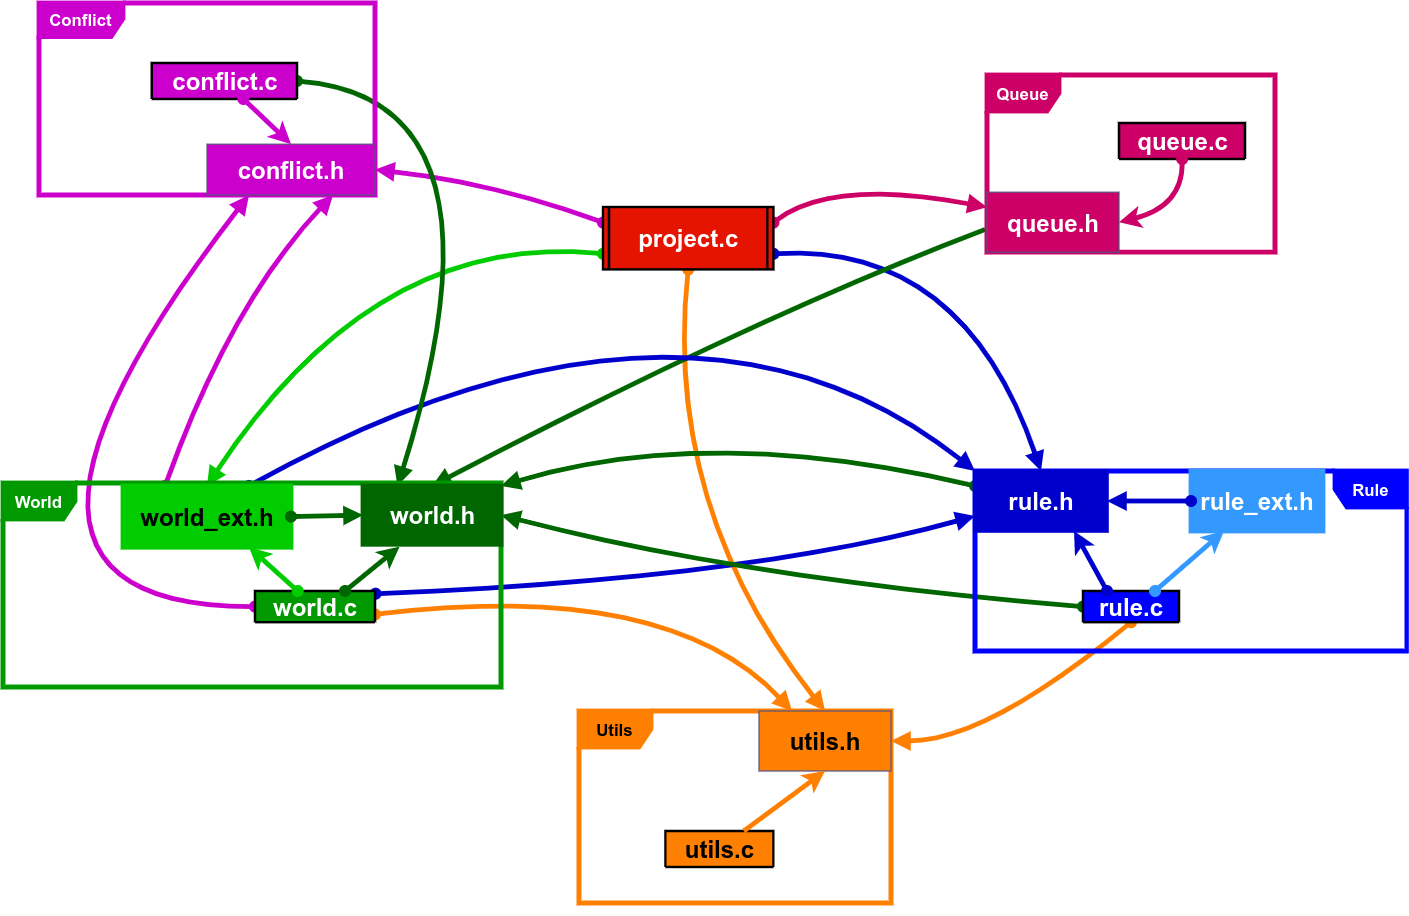
\includegraphics[width=\textwidth]{src.png}
        \caption{Dépendances des sources}
        \label{fig:GrapheDepSource}
    \end{subfigure}
    
    \bigskip
    
    \begin{subfigure}{0.8\textwidth}
        \centering
        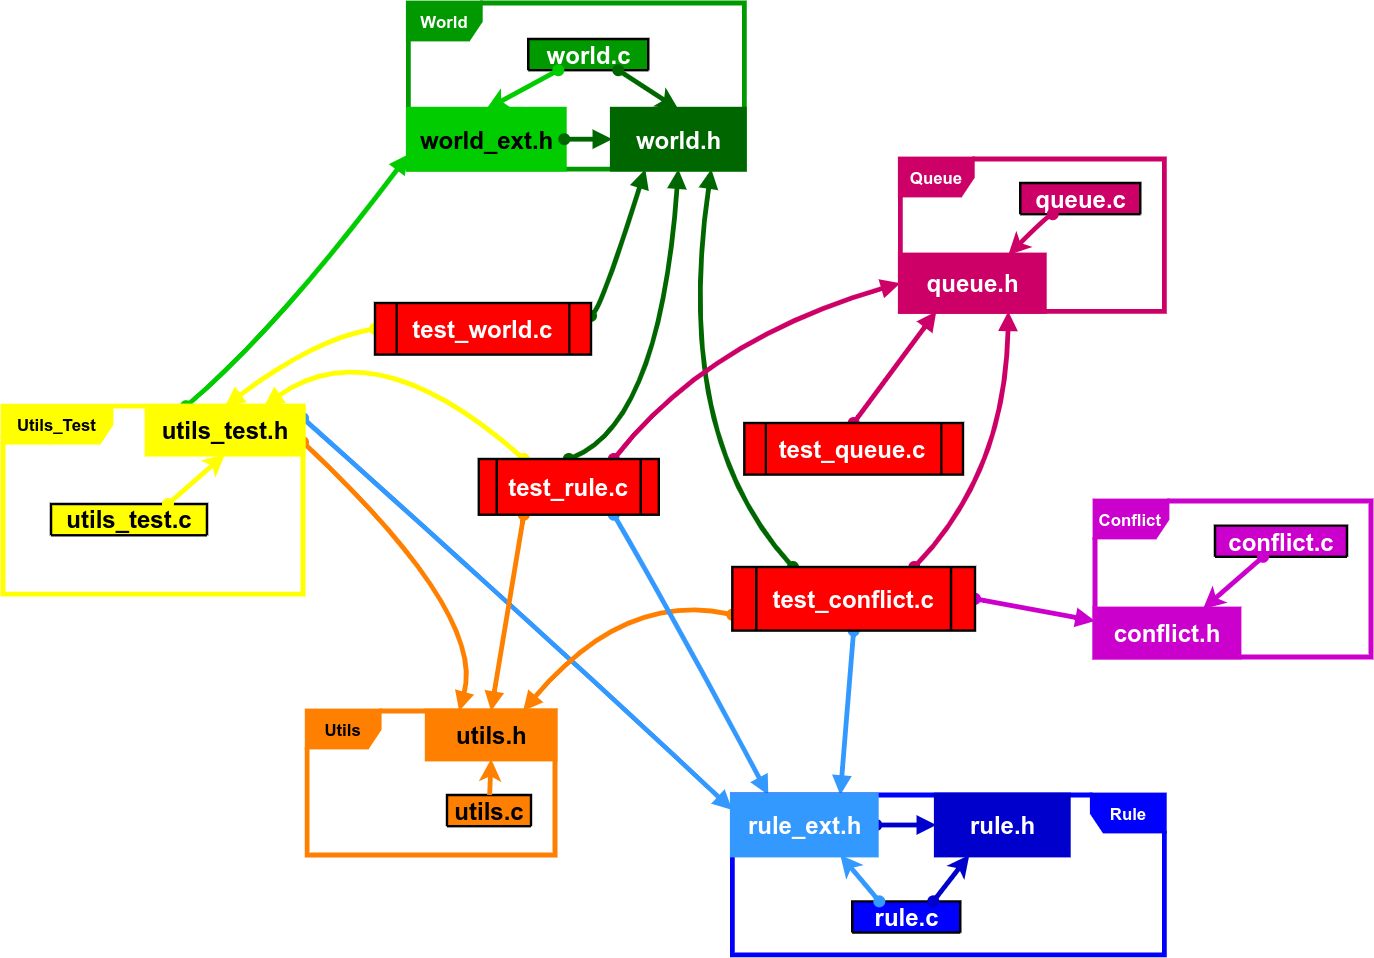
\includegraphics[width=\textwidth]{tst.png}
        \caption{Dépendances des tests}
        \label{fig:GrapheDepTests}
    \end{subfigure}
    \caption{Graphes des dépendances du projet}
    \label{fig:GrapheDep}
\end{figure}